\documentclass[main.tex]{subfiles}
\begin{document}

\chapter{Quantum Information}

\section{The basics}

\paragraph{Qubit}

It can be physically realized with any two-state system.
It is a complex superposition of \(\ket{0} \) and \(\ket{1} \). Thanks to normalization and \(U(1)\) gauge invariance (a ket is defined up to a phase) we can always make \(\ket{0} \)'s coefficient real and \(\in [0,1]\): the ket can always be written as

\begin{equation} \label{eq:qubit}
    \ket{\psi} = \cos(\frac{\theta}{2}) \ket{0} + \sin(\frac{\theta}{2}) e^{ i  \varphi} \ket{1}
\end{equation}

with \(\varphi \in [0,2 \pi]\) and \(\theta \in [0, \pi]\): these can be interpreted as angles on a sphere. The fact that \(\theta\) is divided by two comes from the coordinates we choose in \(S^3 \subset \C^2\).

We can use an \(n\)-qubit system:

\begin{equation} \label{eq:n-qubit-state}
    \ket{\psi } = \sum _{i=0} ^{2^n-1} a_i \ket{i}
\end{equation}

where \(\ket{i} \) is a base state of the tensor product space of the \(n\) Hilbert spaces: \(\ket{i} = \ket{\alpha_0}_0 \otimes \ket{\alpha_1}_1 \otimes \dots \ket{\alpha_{n-1}}_{n-1} \); the \(\alpha_j\) are the components of the representation of \(i\) in binary: \(\alpha_0 \alpha_1 \dots \alpha_{n-1}\) (with \(\alpha_j =0,1\)). This is called the \emph{computational basis}.

We assume the state to be normalized: \(\sum _{i}  \abs{a_i} ^2 = 1 \)

\paragraph{Entanglement}

A state \(\ket{\psi } \) is called \emph{entangled} if there are no subsystem kets \(\ket{\psi _i} _i\), \(i = A, B\) such that \(\ket{\psi } = \ket{\psi _A} _A \otimes \ket{\psi _B} _B\).

\section{Quantum gates}
They are unitary trasformations: \(U: \H \rightarrow \H\), \(U ^\dag U = UU^\dag= \mathbb{1}\).

They can be decomposed into smaller gates, which are in general \(2n \times 2n\) complex unitary matrices, but we will usually just use \(n=1, 2\).

If two gates are represented by \(2 \times 2\) matrices, indexed in the computational basis as \(A_i ^j\) and \(B_k^l\) with \(i, j, k, l = 0,1\),  then their tensor product will be

\begin{equation}
    [A_i^j B_k^l] = [A \otimes B]_i^j\,_k^l = [A \otimes B ] _M ^N
\end{equation}

where we grouped the indices \(ik = M\) and \(jl=N\), in order to write two-component fourth order tensors as four-dimensional order two matrices. What are \(M\) and \(N\)  then? \(i, j\) and so on are binary digits, so it is natural to interpret \(M\) and \(N\) as numbers between \(0\) and \(3\) written in binary.
Of course, this can be generalized to any order, keeping the same pattern, and be applied to vectors as well.

\paragraph{Hadamard} \label{par:hadamard}
It is a \emph{one-qubit gate} which switches from the computational basis to the eigenstates of \(\sigma_z\), which we call \(\ket{+} = H \ket{0} \propto \ket{0} +\ket{1}   \) and \(\ket{-} = H \ket{1} \propto \ket{0} - \ket{1} \).

\begin{equation}
    H = \frac{1}{\sqrt{2} } \begin{pmatrix}
    1   & 1 \\
    1   & -1
    \end{pmatrix}
\end{equation}

We can also express it, for the basis states, as \(H \ket{x} = \sqrt{1/2} \sum _{y=0}^1 (-)^{xy} \ket{y}  \).

\paragraph{Phase}
It is a \emph{one-qubit gate} which  gives a phase to a state: applying it to a generic qubit, written as \eqref{eq:qubit}, we get \(R_z(\delta) \ket{\psi} =  \cos(\theta/2) \ket{0} + \exp(i(\varphi+\delta)) \sin(\theta/2)\ket{1}\).

\begin{equation} \label{eq:phase-gate}
    R_z (\delta) = \exp(i \delta \sigma_z) = \begin{pmatrix}
    1   & 0 \\
    0   & \exp(i \delta)
    \end{pmatrix}
\end{equation}

\paragraph{Control not} \label{par:cnot}
It is a \emph{two-qubit gate}  which cannot be written as a tensor product of one-qubit gates.

\begin{equation}
    \text{CNOT} = \begin{pmatrix}
    1   &  0 &   &  \\
      0 & 1  &   &  \\
       &   & 0  & 1 \\
       &   & 1  & 0
    \end{pmatrix}
\end{equation}

It generates entanglement: let us apply it to the separable state \(\alpha \ket{00} + \beta \ket{10} \): it returns \(\alpha \ket{00} + \beta \ket{11} \), which is entangled.

\paragraph{Control phase}

It is a \emph{two-qubit gate}:

\begin{equation}
    \text{CPHASE}(\delta) = \begin{pmatrix}
    \mathbb 1   & 0 \\
    0   & R_z(\delta)
    \end{pmatrix}
\end{equation}

where we used the phase gate \eqref{eq:phase-gate}.

\begin{bluebox}
It can be written as \(\text{CPHASE} (\delta) = [\mathbb 1 \otimes R_z(\delta/2)] [\text{CNOT}] [\mathbb 1 \otimes R_z(-\delta/2)] [\text{CNOT}] [ R_z(\delta/2) \otimes\mathbb 1 ]\): the steps  (multiplying from right to left, starting from just \([ R_z(\delta/2) \otimes\mathbb 1 ]\)) are as follows:

\begin{multline}
    \begin{pmatrix}
    1   &   &   &  \\
       & 1  &   &  \\
       &   & e^{i \delta/2}  &  \\
       &   &   & e^{i \delta /2}
    \end{pmatrix}
\rightarrow
    \begin{pmatrix}
    1   &   &   &  \\
       & 1  &   &  \\
       &   &  & e^{i \delta/2}  \\
       &   &   e^{i \delta /2} &
    \end{pmatrix}
\rightarrow
    \begin{pmatrix}
    1   &   &   &  \\
       & e^{-i \delta/2}  &   &  \\
       &   &  & e^{i \delta/2}  \\
       &   &   1 &
    \end{pmatrix}
\rightarrow
\\
\rightarrow
    \begin{pmatrix}
    1   &   &   &  \\
       & e^{-i \delta/2}  &   &  \\
       &   &  1 &  \\
       &   &    & e^{i \delta/2}
    \end{pmatrix}
\rightarrow
    \begin{pmatrix}
    1   &   &   &  \\
       & 1  &   &  \\
       &   &  1 &  \\
       &   &    & e^{i \delta}
    \end{pmatrix}
\end{multline}
\end{bluebox}

\begin{bluebox}
We can get any state \(\ket{\psi }\) written as \eqref{eq:qubit} with Hadamard and phase-shift:

\begin{subequations}
\begin{align}
  \ket{\psi }  &= R_z(\pi/2 + \varphi) H R_z(\theta) H\ket{0}  \\
  &= \frac{1}{2} \begin{pmatrix}
    1 + e^{i \theta} \\
     i  \qty(e^{i \varphi}  - e^{i (\theta + \varphi)})
  \end{pmatrix}  \\
  &= \label{eq:sub-gate-phase}
  \frac{1}{2} \begin{pmatrix}
    e^{i \theta /2} + e^{-i \theta /2} \\
    i^{-1} \qty(e^{i \theta/2} - e^{-i \theta/2}) e^{i \varphi}
\end{pmatrix}  \\
 &= \begin{pmatrix}
 \cos(\theta/2)  \\
 \sin(\theta/2) e^{i \varphi}
 \end{pmatrix}
\end{align}
\end{subequations}

where in the step \eqref{eq:sub-gate-phase} we used the fact that a quantum state is only defined up to a phase, and multiplied by \(\exp(-i \theta/2) \).
\end{bluebox}


\paragraph{Binary function unitarity}

In general a function \(f: \qty{0,1}^n \rightarrow \qty{0,1}\) will not be injective, therefore it will not be unitary. In order to represent it as unitary we must "carry over" the input:

\begin{equation}
    U_f \ket{x} \ket{0} = \ket{x} \ket{f(x)}
\end{equation}

in order to have a more general trasformation we define it for arbitrary input on the second system:

\begin{equation}
    U_f \ket{x} \ket{y} = \ket{x} \ket{y \oplus f(x)}
\end{equation}

where \(\oplus\) is bitwise XOR.

\paragraph{Parallelism}

We can do lots of computation with a single gate: say we have a state like \eqref{eq:n-qubit-state}, then

\begin{equation}
    U_f \sum _{x=0}^{2^n-1} a_x \ket{x} \ket{y}  = \sum _{x=0}   ^{2^n-1} a_x \ket{x} \ket{y \oplus f(x)}
\end{equation}

For this to be really different from classical computing, however, a significant portion of the \(2^n\) coefficients \(a_x\) must be nonzero. We now will show how to produce the state in which they are all equal to \(2^{-n/2}\), assuming we can produce \(\ket{0} ^{\otimes n}\). We apply a \nameref{par:hadamard} gate to every qubit, which carries a normalization and a factor of \((-)^{x_i y_i}\), so we get:

\begin{equation}
    H ^{\otimes n} \ket{x} = \frac{1}{\sqrt{2^n} } \sum _{y=0}   ^{2^n -1} (-)^{x\cdot y} \ket{y}
\end{equation}

And the desired state can be found by setting \(x = 0\). Do note that while this looks "entangled" we found it by applyng single-qubit gates: it is still separable (we can see this from the fact that its density matrix has the same value in every entry, so its rank is 1).

\paragraph{No cloning}

A  \emph{general}  cloning unitary operator would look like: \(U \ket{x} \ket{0} = \ket{x} \ket{x} \).
Let us assume we have one, and let us apply it to two different states: \(A = U\ket{\psi}\ket{0}=\ket{\psi} \ket{\psi }  \) and \(B = U\ket{\varphi} \ket{0} = \ket{\varphi} \ket{\varphi} \). Now, let us compute the scalar product of \(A\) and \(B\):

\begin{subequations}
\begin{align}
  A \cdot B &= \bra{\psi} \bra{0} U^\dag  U\ket{\varphi} \ket{0}  \\
  &= \braket{\psi}{\varphi} \braket{0}{0} U^\dag U  \\
  &= \braket{\psi}{\varphi}
\end{align}
\end{subequations}

but also

\begin{subequations}
\begin{align}
  A \cdot B &= \bra{\psi} \bra{\psi}  \ket{\varphi} \ket{\varphi}   \\
  &= \braket{\psi}{\varphi}^2
\end{align}
\end{subequations}

and in general \(\braket{\psi}{\varphi} \neq 0,\pm 1\), so we found a contradiction. Note that we \emph{can} create a partial cloning machine which works only on the basis states of some basis: we extend by linearity the desired cloning. If we want to clone the computational basis, the gate is the CNOT (see \Nameref{par:cnot}).

\begin{bluebox}
  Alternative proof: apply \(U (\ket{x} + \ket{y}) \otimes \ket{0} = (\ket{x} + \ket{y}) ^{\otimes 2} \) (a separable state), but \(U\) must be linear, so \(U (\ket{x} + \ket{y}) \otimes \ket{0} = \ket{x} \ket{x} + \ket{y} \ket{y} \), generally an entangled state.
\end{bluebox}

\section{Miscellaneous concepts}

\subsection{Algorithmic complexity}

We can distinguish algorithms by how many resources (computation time, RAM, ...) they require:

\begin{enumerate}
    \item \(P\): classical polynomial time;
    \item \(NP\): classical nondeterministic polynomial time: there exists a nondeterministic Turing machine\footnote{Same as a regular Turing machine, except that in a certain configuration it can have different actions, and in a certain sense it ``tries them all''.} which finds the solution in polynomial time --- the solution can thus be verified in polynomial time;
    \item \(NP-\text{hard}\): problems to which every \(P\) problem can be reduced in polynomial time;
    \item \(NPC\): \(NP\) problems which are also \(NP-\text{hard}\);
    \item \(BPP\): bounded error probabilistic polynomial: it can give us the correct answer in polynomial time with probability \(\P>1/2\).
    \item \(BQP\): bounded error quantum polynomial: it is a quantum algorithm which can give us the correct answer in polynomial time with probability \(\P>1/2\).
\end{enumerate}

Surely \(P \subseteq BPP \subseteq BQP\). We are not sure whether \(BQP \subseteq BPP\).

\subsection{Fidelity}

We introduce a notion of distance between states:

\begin{equation}
    F = \abs{\braket{\psi_1}{\psi_2} }^2
\end{equation}

\(F\) is monotonous in \(\norm{\ket{\psi_1} - \ket{\psi _2} }_2\).
\(F\) is also the \(\cos^2(\theta/2) \), where \(\theta\) is the angle between the two vectors in Bloch space.

\begin{bluebox}
  Let us prove these two statements: first of all notice that \(\norm{\ket{\psi_1} - \ket{\psi _2} }_2 = \sqrt{2 - 2 \Re \braket{\psi_1}{\psi_2}}\).
  Now, the scalar product \(\braket{\psi_1}{\psi_2}\) is in general a complex number but we can rotate the starting functions by an arbitrary phase, making it real and positive. So we get \(\Re \braket{\psi_1}{\psi_2} = \abs{\braket{\psi_1}{\psi_2}}  = \sqrt{F} \). Then, we can see that

  \begin{equation} \label{eq:norm-of-difference-fidelity}
    \norm{\ket{\psi_1} - \ket{\psi _2} }_2 = \sqrt{2(1-\sqrt{F})}
  \end{equation}

  Now, we want to prove \(F = \cos^2(\theta/2) \): let \(U\) be a unitary transformation which maps \(\ket{\psi _1} \) to \(\ket{0}\). We can rewrite \(F = \abs{\bra{\psi_1} U^\dag U \ket{\psi_2}}^2\). We can expand the applications of \(U\) to the vectors to get \(\abs{\bra{0} \qty(\alpha \ket{0} + \beta \ket{1} ) }^2\).

  Now, since states are always defined up to a phase, we can pick \(\alpha\) to be real and positive. Then we have put the state \(U \ket{\psi_1}\) in the canonical form \eqref{eq:qubit}, and the result follows.
\end{bluebox}

\begin{figure}
    \centering
    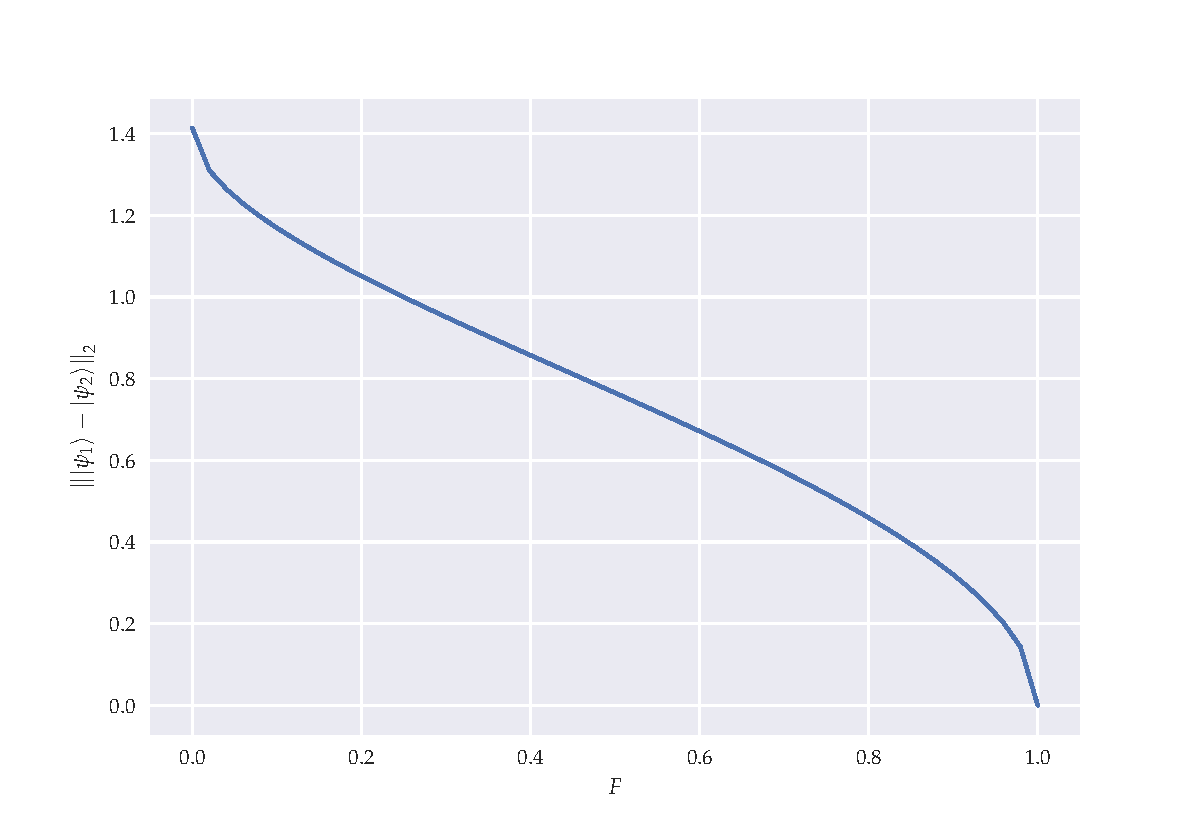
\includegraphics[width=0.7\textwidth]{figures/Fidelity.pdf}
    \caption{Norm of difference vs fidelity: a plot of equation \eqref{eq:norm-of-difference-fidelity}}
    \label{fig:fidelity}
\end{figure}

\section{Quantum teleportation}

It is possible to clone a generic quantum state \(\ket{\psi } = \alpha \ket{0} + \beta \ket{1}  \) assuming we start with two entangled qubits, one in the starting location and one at the destination: so, if these two qubits are called \(A\) and \(B\) and the state we want to transmit is in subsystem \(C\), we start with

\begin{equation}
    \qty(\frac{\ket{00} + \ket{11} }{\sqrt{2} })_{AB} \otimes \ket{\psi}_C
\end{equation}

The protocol is this:

\begin{enumerate}
    \item Apply the gate \(\text{C}_C\text{NOT}_A\); \label{step:cnot}
    \item apply the gate \(H_C\); \label{step:hadamard}
    \item measure \(A\) and \(C\) in the computational basis: call the result \(x\);
    \item apply a gate \(V_x\), selected according to table \ref{tab:teleportation-gate}, to \(B\).
\end{enumerate}

\begin{table}[H]
    \centering
    \begin{tabular}{c|c}
        \(x\) & \(V_x\) \\
        \hline
        00 & \(\mathbb 1\) \\
        01 & \(\sigma_z\) \\
        10 & \(\sigma_x\) \\
        11 & \(\sigma_z \sigma_x\)
    \end{tabular}
    \caption{Possibilities for gate \(V_x\). }
    \label{tab:teleportation-gate}
\end{table}

\begin{greenbox}
  Possibly, when Montangero wrote \(AC=01\) he meant \(A=1\) and \(C=0\).
\end{greenbox}

We can realize all of this with the gates \(\text{CNOT}\), Hadamard and \(\sigma_z\) (we can recover \(\sigma_x\) as \(\sigma_x = H \sigma_z H\).

\section{Quantum interferometry}

\paragraph{Beam splitter}

We call the sides of the BS \(A\) and \(B\), and denote the absence or presence of light on either side by \(\ket{0,1} _{A, B}\). Then the action of the beam splitter is unitary and can be represented in the partial basis \(\ket{0}_A \otimes \ket{1} _B , \ket{1}_A \otimes \ket{0} _B\) as

\begin{equation}
    U_{BS} = \frac{1}{\sqrt{2} }
    \begin{pmatrix}
    1   & i \\
    i   & 1
    \end{pmatrix}
\end{equation}

Note that \(U_{BS}^2 = i\sigma_x\) in the BS-side basis: if we build a Mach-Zender interferometer, that is, we chain two beam-splitters, the light from the two paths interferes and we get some only on one side of the BS (the side opposite of the starting one).

\paragraph{Bomb detection}

If we block one of the paths between the detectors, around half of the time the light will hit this obstacle (our `bomb'). Around half the time it will go to the second BS, and then a quarter of the time it will be detected on either side of the BS. On the other hand, if there is no obstacle, we will see photons \emph{only} on a certain side of the final BS.

So around \(\frac[i]{1}{4} \) of the time we will have detected the bomb without the photon actually \emph{having been there}.

\section{Zeno effect}

We will with \(\hbar=1\).
We look of the \emph{survival probability} with which we will retain our starting state: if our evolution operator is \(U = \exp(-iHt) \), this probability is \(\P = A^*A\), where \(A = \braket{\psi_0}{\psi (t)} \) and \(\ket{\psi (t)} = U \ket{\psi _0} \).

How does this probability look like for small \(t\)? We can expand, for a small \(\delta{t}\):

\begin{equation}
    U \sim \mathbb 1 -i H \delta{t} - H^2 \delta t^2
\end{equation}

then we will have

\begin{equation}
    A = \bra{\psi_0}  \qty(\mathbb 1 -i H \delta{t} - H^2 \delta t^2) \ket{\psi_0}
    = 1 -i \expval{H}_0 \delta{t} - \frac{1}{2}  \expval{H^2} _0 \delta t^2
\end{equation}

so we can calculate \(\P\):

\begin{equation} \label{eq:zeno-probability}
    \P = \abs{1 -i \expval{H}_0 \delta{t} - \frac{1}{2} \expval{H^2} _0 \delta t^2}^2
    = 1 - \delta t^2 \qty(\expval{H^2} _0 - \expval{H}_0^2)
\end{equation}

Equation \eqref{eq:zeno-probability} is accurate to the order \(\delta t^3\), since we only ignored a fourth order term. The term multiplying \(\delta t^2\) can be interpreted as the inverse of a characteristic time:

\begin{equation}
    \tau = \frac{1}{\sqrt{\expval{H^2} _0 - \expval{H}_0^2}} = \frac{1}{\Delta H _0}
\end{equation}

\paragraph{Repeated measurements}

If we measure some observable with \(\ket{\psi _0}\) as an eigenspace, a fraction \(\frac[i]{t^2}{\tau^2} \) of the time we will get something different from \(\ket{\psi _0} \).

So, if in a long time \(t\) we measured \(N\) times, the probability of the system having remained in the original state is at least \(\P (t) \geq \P^N(\frac[i]{t}{N} )\): we consider the case in which the system remained in the state for \emph{all} the measurements. The latter pertains to a small time so we can apply equation \eqref{eq:zeno-probability}:

\begin{equation}
    \P \geq \P^N(\frac{t}{N}) = \qty(1- \frac{t^2}{N^2 \tau^2} )^N
\end{equation}

if we fix the measurement rate \(\frac[i]{N}{t} = R\) this becomes \(\P \geq x^t\), with \(x = \qty(1 - \frac[i]{1}{R^2\tau^2})^R\).

\section{Non-unitary evolution}

It happens when the particle can escape the system; for example in optical systems there can be a complex index of refraction. The Hamiltonian will look like

\begin{equation}
    H = H_0 - iV \mathbb 1
\end{equation}

where \(V \in \R^+\). The unitary evolution has an \(i\) multiplying the Hamiltonian, so we get a decreasing real exponential.

We will have \(A \sim 1 -V \delta t + O(\delta t^2)\), so \(\P  \sim 1 - 2V \delta t + O(\delta t^2)\): the first derivative is nonzero!

\end{document}
